%==============================================================================
% Chapitre 27 - Centre de pression
%==============================================================================

\section{Introduction}

Lorsqu'un projectile traverse l'air, il subit de nombreuses forces
aérodynamiques.

Ces forces résultent de l'interaction entre le projectile et l'écoulement
d'air qui l'entoure.

Pour simplifier leur étude, il est pratique de remplacer l'ensemble de ces
forces par une force unique appliquée en un point particulier.

Ce point est appelé centre de pression.

\begin{aretenir}

Le centre de pression est le point d'application résultant des forces
aérodynamiques agissant sur le projectile.

\end{aretenir}

\section{Définition}

Le centre de pression, souvent noté CP, est le point où l'on peut considérer
que s'applique la résultante des forces aérodynamiques.

Il dépend notamment :

\begin{itemize}
    \item de la géométrie du projectile ;
    \item de son incidence ;
    \item du régime d'écoulement ;
    \item du nombre de Mach.
\end{itemize}

Contrairement au centre de gravité, le centre de pression n'est pas
nécessairement fixe.

\begin{figure}[htbp]
\centering
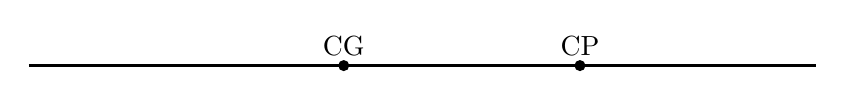
\begin{tikzpicture}

\draw[thick] (0,0) -- (10,0);

\fill (4,0) circle (2pt);
\fill (7,0) circle (2pt);

\node[above] at (4,0) {CG};
\node[above] at (7,0) {CP};

\end{tikzpicture}
\caption{Position relative du centre de gravité et du centre de pression.}
\label{fig:cg_cp}
\end{figure}

\section{Analogie intuitive}

Une girouette constitue un excellent exemple.

La surface exposée au vent crée une force aérodynamique.

Cette force agit à une certaine distance de l'axe de rotation.

Cette disposition provoque naturellement l'orientation de la girouette face
au vent.

Le même principe intervient pour les projectiles.

\section{Centre de gravité et centre de pression}

Le centre de gravité et le centre de pression sont deux notions distinctes.

\begin{itemize}
    \item Le centre de gravité dépend de la répartition des masses.
    \item Le centre de pression dépend de l'écoulement de l'air.
\end{itemize}

Les deux points peuvent être éloignés l'un de l'autre.

Cette distance joue un rôle majeur dans la stabilité.

\section{Projectile parfaitement aligné}

Lorsqu'un projectile est parfaitement aligné avec sa trajectoire :

\begin{itemize}
    \item les forces latérales sont faibles ;
    \item les moments aérodynamiques sont réduits ;
    \item le centre de pression joue un rôle discret.
\end{itemize}

La situation change dès qu'une perturbation apparaît.

\section{Incidence}

L'incidence correspond à l'angle entre :

\begin{itemize}
    \item l'axe du projectile ;
    \item la direction réelle de déplacement.
\end{itemize}

Dès qu'une incidence apparaît, les forces aérodynamiques génèrent des
moments qui tendent à modifier l'orientation du projectile.

\section{Moment aérodynamique}

Lorsque le centre de pression ne coïncide pas avec le centre de gravité,
une force aérodynamique produit un moment.

Ce moment est donné par :

\begin{equation}
M = F \times d
\end{equation}

où :

\begin{itemize}
    \item $M$ est le moment ;
    \item $F$ est la force aérodynamique ;
    \item $d$ est la distance entre le centre de gravité et le centre de
          pression.
\end{itemize}

\section{Position relative des centres}

La position relative du centre de pression par rapport au centre de gravité
est fondamentale.

Deux cas principaux peuvent être rencontrés :

\begin{itemize}
    \item centre de pression derrière le centre de gravité ;
    \item centre de pression devant le centre de gravité.
\end{itemize}

\section{Centre de pression derrière le centre de gravité}

Lorsque le centre de pression est situé derrière le centre de gravité,
l'écoulement tend généralement à réaligner le projectile.

Cette configuration est naturellement stable.

C'est le principe utilisé par :

\begin{itemize}
    \item les flèches ;
    \item les roquettes empennées ;
    \item de nombreux projectiles stabilisés par empennage.
\end{itemize}

\begin{aretenir}

Un projectile dont le centre de pression est situé derrière le centre de
gravité possède généralement une stabilité naturelle.

\end{aretenir}

\section{Centre de pression devant le centre de gravité}

Lorsque le centre de pression se trouve devant le centre de gravité,
une perturbation tend à s'amplifier.

Cette configuration est naturellement instable.

Les projectiles d'armes légères se trouvent souvent dans une situation qui
serait instable sans rotation.

\section{Pourquoi les balles modernes tournent-elles ?}

Les projectiles cylindro-ogivaux modernes possèdent généralement :

\begin{itemize}
    \item un centre de gravité relativement avancé ;
    \item un centre de pression situé de telle sorte qu'une stabilisation
          supplémentaire est nécessaire.
\end{itemize}

Cette stabilisation est obtenue grâce à la rotation imposée par les rayures.

Les chapitres suivants détailleront ce mécanisme.

\section{Déplacement du centre de pression}

Contrairement au centre de gravité, le centre de pression peut se déplacer.

Sa position varie notamment avec :

\begin{itemize}
    \item le nombre de Mach ;
    \item l'incidence ;
    \item la forme du projectile.
\end{itemize}

Ce phénomène complique l'analyse des trajectoires.

\section{Régimes subsonique et supersonique}

La répartition des pressions autour d'un projectile diffère fortement selon
le régime de vol.

Le centre de pression peut donc se déplacer lors du passage :

\begin{itemize}
    \item du régime supersonique ;
    \item au régime transsonique ;
    \item puis subsonique.
\end{itemize}

Ces variations jouent parfois un rôle important dans la stabilité.

\section{Centre de pression et aérodynamique}

Les ingénieurs cherchent généralement à maîtriser la position du centre de
pression.

Ils peuvent agir sur :

\begin{itemize}
    \item la forme de l'ogive ;
    \item la longueur ;
    \item le boat-tail ;
    \item les empennages.
\end{itemize}

Ces paramètres influencent directement le comportement du projectile.

\section{Centre de pression et simulation}

Dans les modèles simples, le centre de pression n'apparaît pas explicitement.

Dans les modèles avancés, il devient indispensable.

Les modèles :

\begin{itemize}
    \item 4DOF ;
    \item 5DOF ;
    \item 6DOF ;
\end{itemize}

utilisent directement sa position ou ses effets.

\begin{simulation}

Les modèles de masse ponctuelle ignorent généralement les notions de centre
de pression et de stabilité aérodynamique.

\end{simulation}

\section{Vers les moments d'inertie}

Nous connaissons désormais :

\begin{itemize}
    \item le centre de gravité ;
    \item le centre de pression.
\end{itemize}

Pour comprendre la réaction du projectile aux moments aérodynamiques, il
reste à étudier la manière dont sa masse est répartie autour de ses axes.

Cette étude conduit naturellement à la notion de moment d'inertie.

\section{À retenir}

\begin{aretenir}

\begin{itemize}
    \item Le centre de pression représente l'action résultante de l'air sur
          le projectile.
    \item Il est distinct du centre de gravité.
    \item La distance CG--CP crée des moments aérodynamiques.
    \item La position relative de ces deux points conditionne la stabilité.
    \item Le centre de pression peut se déplacer selon les conditions de vol.
\end{itemize}

\end{aretenir}
